%% Exemplo de utilizacao do estilo de formatacao abnt-UTFPR.cls para LaTeX (v1.3)
%% Autores: Hugo Vieira Neto (hvieir@utfpr.edu.br)
%%          Diogo Rosa Kuiaski (diogo.kuiaski@gmail.com)

%% Modificado (27-11-2010) por Adolfo Neto (http://adolfoneto.wikidot.com)

\documentclass{abnt-UTFPR} % estilo de documento abnTeX
\usepackage[alf,abnt-emphasize=bf,bibjustif,recuo=0cm]{abntcite} % estilo de bibliografia abnTeX
\usepackage[brazil]{babel} % pacote portugues brasileiro
\usepackage[latin1]{inputenc} % pacote para acentuacao direta
\usepackage{amsmath,amsfonts,amssymb} % pacote matematico
\usepackage{graphicx} % pacote grafico
\usepackage{times} % fonte times

% ---------- Preambulo ----------
\instituicao{Universidade Tecnol�gica Federal do Paran�} % nome da instituicao
\programa{Programa de P�s-gradua��o em Computa��o Aplicada} % nome do programa
\area{Engenharia de Sistemas Computacionais} % [Engenharia Biom\�dica] ou [Inform\'atica Industrial] ou [Telem\�tica]

\documento{Disserta��o} % [Disserta\c{c}\~ao] ou [Tese]
\nivel{Mestrado} % [Mestrado] ou [Doutorado]
\titulacao{Mestre} % [Mestre] ou [Doutor]

\titulo{T�tulo em Portugu�s} % titulo do trabalho em portugues
\title{Title in English} % titulo do trabalho em ingles

\autor{Nome do Autor} % autor do trabalho
\cita{SOBRENOME, Nome} % sobrenome (maiusculas), nome do autor do trabalho

\palavraschave{Palavra-chave 1, Palavra-chave 2, ...} % palavras-chave do trabalho
\keywords{Keyword 1, Keyword 2, ...} % palavras-chave do trabalho em ingles

\comentario{\UTFPRdocumentodata\ apresentada ao \UTFPRprogramadata\ da \ABNTinstituicaodata\ como requisito parcial para obten\c{c}\~ao do t\'itulo de ``\UTFPRtitulacaodata\ em Ci\^encias'' -- \'Area de Concentra\c{c}\~ao: \UTFPRareadata.}

\orientador{Nome do Orientador} % nome do orientador do trabalho
%\orientador[Orientadora:]{Nome da Orientadora} % <- no caso de orientadora, usar esta sintaxe
\coorientador{Nome do Co-orientador} % nome do co-orientador do trabalho, caso exista
%\coorientador[Co-orientadora:]{Nome da Co-orientadora} % <- no caso de co-orientadora, usar esta sintaxe

\local{Curitiba} % cidade
\data{2010} % ano


%---------- Inicio do Documento ----------
\begin{document}

\capa % geracao automatica da capa
\folhaderosto % geracao automatica da folha de rosto
%\termodeaprovacao % <- ainda a ser implementado corretamente

% dedicat�ria (opcional)
\begin{dedicatoria}
Texto da dedicat\'oria.
\end{dedicatoria}

% agradecimentos (opcional)
\begin{agradecimentos}
Texto dos agradecimentos.
\end{agradecimentos}

% epigrafe (opcional)
\begin{epigrafe}
Texto da ep\'igrafe.
\end{epigrafe}

%resumo
\begin{resumo}
Texto do resumo (m\'aximo de 500 palavras).
\end{resumo}

%abstract
\begin{abstract}
Abstract text (maximum of 500 words).
\end{abstract}

% listas (opcionais, mas recomenda-se a partir de 5 elementos)
\listadefiguras % geracao automatica da lista de figuras
\listadetabelas % geracao automatica da lista de tabelas
\listadesiglas % geracao automatica da lista de siglas
\listadesimbolos % geracao automatica da lista de simbolos

% sumario
\sumario % geracao automatica do sumario


%---------- Inicio do Texto ----------
% recomenda-se a escrita de cada capitulo em um arquivo texto separado (exemplo: intro.tex, fund.tex, exper.tex, concl.tex, etc.) e a posterior inclusao dos mesmos no mestre do documento utilizando o comando \input{}, da seguinte forma:
%%---------- Primeiro Capitulo ----------
\chapter{Introdu\c{c}\~ao}
\label{chap:intro}

O presente documento \'e um exemplo de uso do estilo de formata\c{c}\~ao \LaTeX\ elaborado para atender \`as Normas para Elabora\c{c}\~ao de Trabalhos Acad\^emicos da UTFPR. O estilo de formata\c{c}\~ao {\ttfamily normas-utf-tex.cls} tem por base o pacote \textsc{abn}\TeX~-- cuja leitura da documenta\c{c}\~ao \cite{abnTeX2009} \'e fortemente sugerida~-- e o estilo de formata\c{c}\~ao \LaTeX\ da UFPR.

Para melhor entendimento do uso do estilo de formata\c{c}\~ao {\ttfamily normas-utf-tex.cls}, aconselha-se que o potencial usu\'ario analise os comandos existentes no arquivo \TeX\ ({\ttfamily modelo\_*.tex}) e os resultados obtidos no arquivo PDF ({\ttfamily modelo\_*.pdf}) depois do processamento pelo software \LaTeX\ + \textsc{Bib}\TeX~\cite{LaTeX2009,BibTeX2009}. Recomenda-se a consulta ao material de refer\^encia do software para a sua correta utiliza\c{c}\~ao~\cite{Lamport1986,Buerger1989,Kopka2003,Mittelbach2004}.

% Trecho extraído do modelo http://www2.dainf.ct.utfpr.edu.br/ppgca/estrutura-academica/regulamentacao/avaliacao/copy_of_ModeloProjetoeSeminarios.doc/view
A redação do plano de pesquisa ou proposta deve refletir o poder de síntese do seu autor. Utilize as formatações de página, espaçamento e fonte aqui apresentados (Fonte Arial 12, espaçamento entre linhas 1,5, folha tamanho A4, margens padrão do Word). 
Deve haver especial atenção com o índice, pois o mesmo é gerado de maneira automática, não devendo ser apagado. Depois de introduzir todos os seus textos sob os itens apropriados, coloque o cursor do mouse sobre a área onde está o índice, clique com o botão direito do mouse, selecione a opção “Atualizar campo” e depois “Atualizar apenas o número das páginas”. Pronto, o Índice indicará as páginas automaticamente. Não é preciso editá-lo. 
O texto de introdução deve conter três tipos de informações: apresentação do problema, estado da arte e justificativa do projeto. Uma vez que nem sempre é clara a linha divisória entre estes três tópicos, optou-se pela construção de uma seção única de introdução que deverá conter todas as informações acima mencionadas, permitindo ao autor elaborar um texto com fluência lógica e sem redundância de informações.
A apresentação ou formulação do problema deve deixar, de forma bem clara, qual será o objeto de estudo do projeto. As razões para a escolha do tema deverão ser justificadas e, para isso, você deverá discorrer sobre a importância do estudo, quais as possíveis repercussões, quais hipóteses a serem verificadas, etc. 
O estado da arte serve para embasar tanto a formulação do problema como sua justificativa. É preciso situar historicamente a evolução do tema, quais as abordagens já investigadas, qual o estágio atual do conhecimento sobre o assunto ou quais as tendências que se apresentam.
A justificativa do projeto deve indicar por que o projeto deve ser feito. Descreva os fatores de motivação que o levaram a abordar e trabalhar no assunto.
As maneiras mais comuns de citações são a indireta e a direta. Na citação indireta, o texto é criado com base na obra de autor consultado, no qual se reproduz o conteúdo e as idéias do documento original. Exemplo, utilizando Sobrenome do Autor (data), quando o nome do autor faz parte do texto: Segundo Souza (1999), a importância do tema [...]. Exemplo, utilizando (SOBRENOME DO AUTOR, ano) quando é citada a síntese de uma informação: A Revolução Industrial modificou definitivamente o cenário urbano (SOUZA, 2001). Na citação direta há a reprodução exata do texto citado entre aspas, como, por exemplo: A justificativa deste comportamento “é resultado da integração entre parasita e hospedeiro, após a conclusão da fase de migração” (SOUZA, 1987). No capítulo Referências, ao final deste documento, há diversos exemplos para apresentação da fonte de uma referência. Dúvidas e maiores detalhes, vide norma ABNT vigente para citações e referências.
Importante: O formato recomendado para as citações e referências é o ABNT. Consulte o orientador para verificar a necessidade de utilização de um formato de citações e de referências diferente, como a norma Vancouver.
Importante: Todos os trabalhos que envolvem seres humanos (inclusive entrevistas) e animais deverão obter aprovação do Comitê de Ética em Pesquisa (CEP) e devem apresentar uma cópia do Termo de Consentimento Informado (TCI), que deve ser assinado pelos participantes da pesquisa. Os requisitos do comitê de ética local estão à disposição no CEP, disponível em http://www.utfpr.edu.br/estrutura-universitaria/pro-reitorias/proppg/comite-de-etica-em-pesquisa-1 . O TCI é o documento em que são informadas aos participantes da pesquisa, em linguagem simples e acessível, todas as implicações possíveis (passadas, presentes ou futuras) da pesquisa para esta pessoa. Ao assinar este termo a pessoa estará autorizando sua inclusão na pesquisa. De modo semelhante, as pesquisas que envolverem animais devem respeitar integralmente os preceitos éticos para experimentação animal. 
O projeto de pesquisa deve estar submetido ao Comitê de Ética em Pesquisa o mais cedo possível, para não inviabilizar os prazos da conclusão do mestrado.
Importante: O Direito Autoral deve ser respeitado. A Constituição da República Federativa do Brasil, em seu Artigo 5, Parágrafo XXVII, indica (BRASIL, 1988): "aos autores pertence o direito exclusivo de utilização, publicação ou reprodução de suas obras, transmissível aos herdeiros pelo tempo que a lei fixar.". A Lei de Direitos Autorais (BRASIL, 1998) afirma:
Art 1º. Esta Lei regula os direitos autorais, entendendo-se sob esta denominação os direitos do autor e os que lhe são conexos.
Art. 7º. São obras intelectuais protegidas as criações de espírito, expressas por qualquer meio ou fixadas em qualquer suporte, tangível ou intangível, conhecido ou que se invente no futuro, como:
I - os textos de obras literárias, artísticas ou científicas;
Art. 22. Pertencem ao autor os direitos morais e patrimoniais sobre a obra que criou.
Art 29. Depende da autorização prévia e expressa do autor a utilização da obra, por quaisquer modalidades, tais como: 
I- a reprodução parcial ou integral;
II- a edição; 
Art. 41. Os direitos patrimoniais do autor perduram por setenta anos contados de 1º de janeiro do ano subsequente ao de seu falecimento, obedecida a ordem sucessória da lei civil.
Art. 46 - Não constitui ofensa aos direitos autorais: 
III - a citação em livros, jornais, revistas ou qualquer outro meio de comunicação, de passagens de qualquer obra, para fins de estudo, crítica ou polêmica, na medida justificada para o fim a atingir, indicando-se o nome do autor e a origem da obra;
A Lei n. 6895, de 17 de dezembro de 1980, que modifica o Código Penal, indica em seu artigo 184 (BRASIL, 1980):
Art. 184 - Violar direito autoral: 
Pena - detenção de 3 meses a 1 ano, ou multa.
§ 1º - Se a violação consistir na reprodução, por qualquer meio, com intuito de lucro, de obra intelectual, no todo ou em parte, sem autorização expressa do autor ou de quem o represente, ou consistir na reprodução de fonograma e videofonograma, sem autorização do produtor ou de quem o represente:
Pena - reclusão de um a quatro anos e multa de Cr\$ 10.000,00 (dez mil cruzeiros) a Cr\$ 50.000,00 (cinqüenta mil cruzeiros).
§ 2º - Na mesma pena do parágrafo anterior incorre quem vende, expõe à venda, aluga, introduz no País, adquire, oculta, empresta, troca ou tem em depósito, com intuito de lucro, original ou cópia de obra intelectual, fonograma ou videofonograma, produzidos com violação de direito autoral.
%-------------------------------------------------------------------------------

\section{Motiva\c{c}\~ao}

Uma das principais vantagens do uso do estilo de formata\c{c}\~ao {\ttfamily normas-utf-tex.cls} para \LaTeX\ \'e a formata\c{c}\~ao \textit{autom\'atica} dos elementos que comp\~oem um documento acad\^emico, tais como capa, folha de rosto, dedicat\'oria, agradecimentos, ep\'igrafe, resumo, abstract, listas de figuras, tabelas, siglas e s\'imbolos, sum\'ario, cap\'itulos, refer\^encias, etc. Outras grandes vantagens do uso do \LaTeX\ para formata\c{c}\~ao de documentos acad\^emicos dizem respeito \`a facilidade de gerenciamento de refer\^encias cruzadas e bibliogr\'aficas, al\'em da formata\c{c}\~ao~-- inclusive de equa\c{c}\~oes  matem\'aticas~-- correta e esteticamente perfeita.

\section{Objetivos}
% Trecho extraído do modelo http://www2.dainf.ct.utfpr.edu.br/ppgca/estrutura-academica/regulamentacao/avaliacao/copy_of_ModeloProjetoeSeminarios.doc/view
Os objetivos devem ser claros, sucintos e diretos. Deve ficar bem evidente qual a pergunta ou questionamento para o qual se busca uma resposta através desta pesquisa. 
Os objetivos são divididos em dois tipos: Objetivo Geral e Objetivos Específicos
%-------------------------------------------------------------------------------

\subsection{Objetivo Geral}
% Trecho extraído do modelo http://www2.dainf.ct.utfpr.edu.br/ppgca/estrutura-academica/regulamentacao/avaliacao/copy_of_ModeloProjetoeSeminarios.doc/view
Como pode ser notado, o título está no singular. Portanto, deve ser apresentado apenas 1 (um) objetivo geral. Aqui deve constar um parágrafo descrevendo esse objetivo.
%-------------------------------------------------------------------------------

Prover um modelo de formata\c{c}\~ao \LaTeX\ que atenda \`as Normas para Elabora\c{c}\~ao de Trabalhos Acad\^emicos da UTFPR~\cite{UTFPR2008} e \`as Normas de Apresenta\c{c}\~ao de Trabalhos Acad\^emicos do DAELN~\cite{DAELN2006}.


\subsection{Objetivos Espec\'ificos}

% Trecho extraído do modelo http://www2.dainf.ct.utfpr.edu.br/ppgca/estrutura-academica/regulamentacao/avaliacao/copy_of_ModeloProjetoeSeminarios.doc/view
O título está no plural. Portanto, espera-se encontrar mais de um objetivo específico neste local. Não confunda objetivo específico com metodologia. Os objetivos específicos são o desdobramento do objetivo geral. 
Pode-se começar esse tópico desta forma: 

Dentre os principais objetivos específicos destacam-se:
Cada objetivo específico será colocado em forma de item e terá uma frase curta, mas que deixe claro qual o objetivo.
A somatória dos objetivos específicos formará o objetivo geral.
%-------------------------------------------------------------------------------

\begin{itemize}
	\item Obter documentos acad\^emicos automaticamente formatados com corre\c{c}\~ao e perfei\c{c}\~ao est\'etica.
	\item Desonerar autores da tediosa tarefa de formatar documentos acad\^emicos, permitindo sua concentra\c{c}\~ao no conte\'udo do mesmo.
	\item Desonerar orientadores e examinadores da tediosa tarefa de conferir a formata\c{c}\~ao de documentos acad\^emicos, permitindo sua concentra\c{c}\~ao no conte\'udo do mesmo.
\end{itemize}

% Trecho extraído do modelo http://www2.dainf.ct.utfpr.edu.br/ppgca/estrutura-academica/regulamentacao/avaliacao/copy_of_ModeloProjetoeSeminarios.doc/view
\section{Estrutura do Trabalho}

Aqui será apresentado a estrutura do trabalho, quantos capítulos e o conteúdo respectivo. O conteúdo de cada capítulo será descrito por uma frase curta e que seja representativa (este item somente será incluído nas versões para qualificação e defesa da dissertação). 
%-------------------------------------------------------------------------------

%\input{fund.tex}
%\input{exper.tex}
%\chapter{Conclus\~ao}
\label{chap:concl}

Espera-se que o uso do estilo de formata\c{c}\~ao \LaTeX\ adequado \`as Normas para Elabora\c{c}\~ao de Trabalhos Acad\^emicos da UTFPR ({\ttfamily normas-utf-tex.cls}) facilite a escrita de documentos no \^ambito desta institui\c{c}\~ao e aumente a produtividade de seus autores. Para usu\'arios iniciantes em \LaTeX, al\'em da bibliografia especializada j\'a citada, existe ainda uma s\'erie de recursos~\cite{CTAN2009} e fontes de informa\c{c}\~ao~\cite{TeX-Br2009,Wikibooks2009} dispon\'iveis na Internet.

Recomenda-se o editor de textos Kile como ferramenta de composi\c{c}\~ao de documentos em \LaTeX\ para usu\'arios Linux. Para usu\'arios Windows recomenda-se o editor \TeX nicCenter~\cite{TeXnicCenter2009}. O \LaTeX\ normalmente j\'a faz parte da maioria das distribui\c{c}\~oes Linux, mas no sistema operacional Windows \'e necess\'ario instalar o software \textsc{MiK}\TeX~\cite{MiKTeX2009}.

Al\'em disso, recomenda-se o uso de um gerenciador de refer\^encias como o JabRef~\cite{JabRef2009} ou Mendeley~\cite{Mendeley2009} para a cataloga\c{c}\~ao bibliogr\'afica em um arquivo \textsc{Bib}\TeX, de forma a facilitar cita\c{c}\~oes atrav\'es do comando {\ttfamily \textbackslash cite\{\}} e outros comandos correlatos do pacote \textsc{abn}\TeX. A lista de refer\^encias deste documento foi gerada automaticamente pelo software \LaTeX\ + \textsc{Bib}\TeX\ a partir do arquivo {\ttfamily reflatex.bib}, que por sua vez foi composto com o gerenciador de refer\^encias JabRef.

O estilo de formata\c{c}\~ao \LaTeX\ da UTFPR e este exemplo de utiliza\c{c}\~ao foram elaborados por Diogo Rosa Kuiaski (diogo.kuiaski@gmail.com) e Hugo Vieira Neto (hvieir@utfpr.edu.br), com contribui\c{c}\~oes de C\'esar Vargas Benitez. Sugest\~oes de melhorias s\~ao bem-vindas.

% Trecho extraído do modelo http://www2.dainf.ct.utfpr.edu.br/ppgca/estrutura-academica/regulamentacao/avaliacao/copy_of_ModeloProjetoeSeminarios.doc/view
As conclusões do trabalho devem ser expostas de maneira clara, lógica e concisa, devendo fundamentar o que foi obtido na discussão. Deverá haver correspondência entre as conclusões e os objetivos específicos propostos no início do trabalho.
Deve haver um relacionamento com a Introdução, onde está a hipótese do trabalho, fechando desta forma o ciclo de desenvolvimento do trabalho. Mais especificamente, as conclusões devem responder aos objetivos específicos.

\section{Trabalhos Futuros}
Indicar aqui os vários trabalhos que podem ser incentivados e realizados a partir deste. Este tópico deve demonstrar que o trabalho desenvolvido não se encerra em si mesmo, mostrando o caminho a ser seguido pelos próximos trabalhos.
%-------------------------------------------------------------------------------


%---------- Primeiro Capitulo ----------
\chapter{Introdu\c{c}\~ao}

O presente documento \'e um exemplo de uso do estilo de formata\c{c}\~ao \LaTeX\ elaborado para atender \`as Normas para Elabora\c{c}\~ao de Trabalhos Acad\^emicos da UTFPR. O estilo de formata\c{c}\~ao {\ttfamily abnt-UTFPR.cls} tem por base o pacote \textsc{abn}\TeX~-- cuja leitura da documenta\c{c}\~ao \cite{abnTeX2009} \'e fortemente sugerida~-- e o estilo de formata\c{c}\~ao \LaTeX\ da UFPR.

Para melhor entendimento do uso do estilo de formata\c{c}\~ao {\ttfamily abnt-UTFPR.cls}, aconselha-se que o potencial usu\'ario analise os comandos existentes no arquivo \TeX\ ({\ttfamily modelo\_*.tex}) e os resultados obtidos no arquivo PDF ({\ttfamily modelo\_*.pdf}) depois do processamento pelo software \LaTeX\ + \textsc{Bib}\TeX~\cite{LaTeX2009,BibTeX2009}. Recomenda-se a consulta ao material de refer\^encia do software para a sua correta utiliza\c{c}\~ao~\cite{Lamport1986,Buerger1989,Kopka2003,Mittelbach2004}.

\section{Motiva\c{c}\~ao}

Uma das principais vantagens do uso do estilo de formata\c{c}\~ao {\ttfamily abnt-UTFPR.cls} para \LaTeX\ \'e a formata\c{c}\~ao \textit{autom\'atica} dos elementos que comp\~oem um documento acad\^emico, tais como capa, folha de rosto, dedicat\'oria, agradecimentos, ep\'igrafe, resumo, abstract, listas de figuras, tabelas, siglas e s\'imbolos, sum\'ario, cap\'itulos, refer\^encias, etc. Outras grandes vantagens do uso do \LaTeX\ para formata\c{c}\~ao de documentos acad\^emicos dizem respeito \`a facilidade de gerenciamento de refer\^encias cruzadas e bibliogr\'aficas, al\'em da formata\c{c}\~ao~-- inclusive de equa\c{c}\~oes  matem\'aticas~-- correta e esteticamente perfeita.

\section{Objetivos}

\subsection{Objetivo Geral}

Prover um modelo de formata\c{c}\~ao \LaTeX\ que atenda \`as Normas para Elabora\c{c}\~ao de Trabalhos Acad\^emicos da UTFPR~\cite{UTFPR2008} e \`as Normas de Apresenta\c{c}\~ao de Trabalhos Acad\^emicos do DAELN~\cite{DAELN2006}.

\subsection{Objetivos Espec\'ificos}

\begin{itemize}
	\item Obter documentos acad\^emicos automaticamente formatados com corre\c{c}\~ao e perfei\c{c}\~ao est\'etica.
	\item Desonerar autores da tediosa tarefa de formatar documentos acad\^emicos, permitindo sua concentra\c{c}\~ao no conte\'udo do mesmo.
	\item Desonerar orientadores e examinadores da tediosa tarefa de conferir a formata\c{c}\~ao de documentos acad\^emicos, permitindo sua concentra\c{c}\~ao no conte\'udo do mesmo.
\end{itemize}


%---------- Segundo Capitulo ----------
\chapter{Desenvolvimento}
\label{chap:desenv}

A seguir ilustra-se a forma de incluir figuras, tabelas, equa\c{c}\~oes, siglas e s\'imbolos no documento, obtendo indexa\c{c}\~ao autom\'atica em suas respectivas listas. A numera\c{c}\~ao sequencial de figuras, tabelas e equa\c{c}\~oes ocorre de modo autom\'atico. Refer\^encias cruzadas s\~ao obtidas atrav\'es dos comandos {\ttfamily \textbackslash label\{\}} e {\ttfamily \textbackslash ref\{\}}. Por exemplo, n\~ao \'e necess\'ario saber que o n\'umero deste cap\'itulo \'e~\ref{chap:desenv} para colocar o seu n\'umero no texto. Isto facilita muito a inser\c{c}\~ao, remo\c{c}\~ao ou reloca\c{c}\~ao de elementos numerados no texto (fato corriqueiro na escrita e corre\c{c}\~ao de um documento acad\^emico) sem a necessidade de renumer\'a-los todos.

\section{Figuras}

Na figura~\ref{fig:dummy} \'e apresentado um exemplo de gr\'afico flutuante. Esta figura aparece automaticamente na lista de figuras. Para uso avan\c{c}ado de gr\'aficos no \LaTeX, recomenda-se a consulta de literatura especializada~\cite{Goossens2007}.

\begin{figure}[!htb]
	\centering
	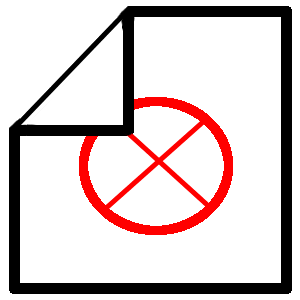
\includegraphics[width=0.2\textwidth]{./figs/dummy.png} % <- formatos PNG, JPG e PDF
	\caption[Exemplo de uma figura]{Exemplo de uma figura onde aparece uma imagem sem nenhum significado especial.}
	\fonte{\cite{abnTeX2009}}
	\label{fig:dummy}
\end{figure}

\section{Tabelas}

Tamb\'em \'e apresentado o exemplo da tabela~\ref{tab:correlacao}, que aparece automaticamente na lista de tabelas. Informa\c{c}\~oes sobre a constru\c{c}\~ao de tabelas no \LaTeX\ podem ser encontradas na literatura especializada~\cite{Lamport1986,Buerger1989,Kopka2003,Mittelbach2004}.

\begin{table}[!htb]
	\centering
	\caption[Exemplo de uma tabela]{Exemplo de uma tabela mostrando a correla\c{c}\~ao entre x e y.}
	\label{tab:correlacao}
	\begin{tabular}{cc}
		\hline 
		x & y \\
		\hline
		1 & 2 \\
		3 & 4 \\
		5 & 6 \\
		7 & 8 \\
		\hline 
	\end{tabular}
	\fonte{Autoria pr\'opria.}
\end{table}

\section{Equa\c{c}\~oes}

A transformada de Laplace \'e dada na equa\c{c}\~ao~(\ref{eq:laplace}), enquanto a equa\c{c}\~ao~(\ref{eq:dft}) apresenta a formula\c{c}\~ao da transformada discreta de Fourier bidimensional\footnote{Deve-se reparar na formata\c{c}\~ao esteticamente perfeita destas equa\c{c}\~oes!}.

\begin{equation}
X(s) = \int\limits_{t = -\infty}^{\infty} x(t) \, \text{e}^{-st} \, dt
\label{eq:laplace}
\end{equation}

\begin{equation}
F(u, v) = \sum_{m = 0}^{M - 1} \sum_{n = 0}^{N - 1} f(m, n) \exp \left[ -j 2 \pi \left( \frac{u m}{M} + \frac{v n}{N} \right) \right]
\label{eq:dft}
\end{equation}

\section{Siglas e s\'imbolos}

O pacote \textsc{abn}\TeX\ permite ainda a defini\c{c}\~ao de siglas e s\'imbolos com indexa\c{c}\~ao autom\'atica atrav\'es dos comandos {\ttfamily \textbackslash sigla\{\}\{\}} e {\ttfamily \textbackslash simbolo\{\}\{\}}. Por exemplo, o significado das siglas\sigla{CPGEI}{Programa de P\'os-gradua\c{c}\~ao em Engenharia El\'etrica e Inform\'atica Industrial},\sigla{DAELN}{Departamento Acad\^emico de Eletr\^onica} e\sigla{UTFPR}{Universidade Tecnol\'ogica Federal do Paran\'a} aparecem automaticamente na lista de siglas, bem como o significado dos s\'imbolos\simbolo{$\lambda$}{comprimento de onda},\simbolo{$v$}{velocidade} e\simbolo{$f$}{frequ\^encia} aparecem automaticamente na lista de s\'imbolos. Mais detalhes sobre o uso destes e outros comandos do \textsc{abn}\TeX\ s\~ao encontrados na sua documenta\c{c}\~ao espec\'ifica~\cite{abnTeX2009}.


%---------- Terceiro Capitulo ----------
\chapter{Conclus\~ao}

Espera-se que o uso do estilo de formata\c{c}\~ao \LaTeX\ adequado \`as Normas para Elabora\c{c}\~ao de Trabalhos Acad\^emicos da UTFPR ({\ttfamily abnt-UTFPR.cls}) facilite a escrita de documentos no \^ambito desta institui\c{c}\~ao e aumente a produtividade de seus autores. Para usu\'arios iniciantes em \LaTeX, al\'em da bibliografia especializada j\'a citada, existe ainda uma s\'erie de recursos~\cite{CTAN2009} e fontes de informa\c{c}\~ao~\cite{TeX-Br2009,Wikibooks2009} dispon\'iveis na Internet.

Recomenda-se o editor de textos Kile como ferramenta de composi\c{c}\~ao de documentos em \LaTeX\ para usu\'arios Linux. Para usu\'arios Windows recomenda-se o editor \TeX nicCenter~\cite{TeXnicCenter2009}. O \LaTeX\ normalmente j\'a faz parte da maioria das distribui\c{c}\~oes Linux, mas no sistema operacional Windows \'e necess\'ario instalar o software \textsc{MiK}\TeX~\cite{MiKTeX2009}.

Al\'em disso, recomenda-se o uso de um gerenciador de refer\^encias como o JabRef~\cite{JabRef2009} ou Mendeley~\cite{Mendeley2009} para a cataloga\c{c}\~ao bibliogr\'afica em um arquivo \textsc{Bib}\TeX, de forma a facilitar cita\c{c}\~oes atrav\'es do comando {\ttfamily \textbackslash cite\{\}} e outros comandos correlatos do pacote \textsc{abn}\TeX. A lista de refer\^encias deste documento foi gerada automaticamente pelo software \LaTeX\ + \textsc{Bib}\TeX\ a partir do arquivo {\ttfamily reflatex.bib}, que por sua vez foi composto com o gerenciador de refer\^encias JabRef.

O estilo de formata\c{c}\~ao \LaTeX\ da UTFPR e este exemplo de utiliza\c{c}\~ao foram elaborados por Diogo Rosa Kuiaski (diogo.kuiaski@gmail.com) e Hugo Vieira Neto (hvieir@utfpr.edu.br), com contribui\c{c}\~oes de C\'esar Vargas Benitez. Sugest\~oes de melhorias s\~ao bem-vindas.


%---------- Referencias ----------
\bibliography{reflatex} % geracao automatica das referencias a partir do arquivo reflatex.bib


%---------- Apendices (opcionais) ----------
\apendice
\chapter{Nome do Ap\^endice}

Use o comando {\ttfamily \textbackslash apendice} e depois comandos {\ttfamily \textbackslash chapter\{\}}
para gerar t\'itulos de ap\^en-dices.


% ---------- Anexos (opcionais) ----------
\anexo
\chapter{Nome do Anexo}

Use o comando {\ttfamily \textbackslash anexo} e depois comandos {\ttfamily \textbackslash chapter\{\}}
para gerar t\'itulos de anexos.

\end{document}
